\documentclass[1p]{elsarticle_modified}
%\bibliographystyle{elsarticle-num}

%\usepackage[colorlinks]{hyperref}
%\usepackage{abbrmath_seonhwa} %\Abb, \Ascr, \Acal ,\Abf, \Afrak
\usepackage{amsfonts}
\usepackage{amssymb}
\usepackage{amsmath}
\usepackage{amsthm}
\usepackage{scalefnt}
\usepackage{amsbsy}
\usepackage{kotex}
\usepackage{caption}
\usepackage{subfig}
\usepackage{color}
\usepackage{graphicx}
\usepackage{xcolor} %% white, black, red, green, blue, cyan, magenta, yellow
\usepackage{float}
\usepackage{setspace}
\usepackage{hyperref}

\usepackage{tikz}
\usetikzlibrary{arrows}

\usepackage{multirow}
\usepackage{array} % fixed length table
\usepackage{hhline}

%%%%%%%%%%%%%%%%%%%%%
\makeatletter
\renewcommand*\env@matrix[1][\arraystretch]{%
	\edef\arraystretch{#1}%
	\hskip -\arraycolsep
	\let\@ifnextchar\new@ifnextchar
	\array{*\c@MaxMatrixCols c}}
\makeatother %https://tex.stackexchange.com/questions/14071/how-can-i-increase-the-line-spacing-in-a-matrix
%%%%%%%%%%%%%%%

\usepackage[normalem]{ulem}

\newcommand{\msout}[1]{\ifmmode\text{\sout{\ensuremath{#1}}}\else\sout{#1}\fi}
%SOURCE: \msout is \stkout macro in https://tex.stackexchange.com/questions/20609/strikeout-in-math-mode

\newcommand{\cancel}[1]{
	\ifmmode
	{\color{red}\msout{#1}}
	\else
	{\color{red}\sout{#1}}
	\fi
}

\newcommand{\add}[1]{
	{\color{blue}\uwave{#1}}
}

\newcommand{\replace}[2]{
	\ifmmode
	{\color{red}\msout{#1}}{\color{blue}\uwave{#2}}
	\else
	{\color{red}\sout{#1}}{\color{blue}\uwave{#2}}
	\fi
}

\newcommand{\Sol}{\mathcal{S}} %segment
\newcommand{\D}{D} %diagram
\newcommand{\A}{\mathcal{A}} %arc


%%%%%%%%%%%%%%%%%%%%%%%%%%%%%5 test

\def\sl{\operatorname{\textup{SL}}(2,\Cbb)}
\def\psl{\operatorname{\textup{PSL}}(2,\Cbb)}
\def\quan{\mkern 1mu \triangleright \mkern 1mu}

\theoremstyle{definition}
\newtheorem{thm}{Theorem}[section]
\newtheorem{prop}[thm]{Proposition}
\newtheorem{lem}[thm]{Lemma}
\newtheorem{ques}[thm]{Question}
\newtheorem{cor}[thm]{Corollary}
\newtheorem{defn}[thm]{Definition}
\newtheorem{exam}[thm]{Example}
\newtheorem{rmk}[thm]{Remark}
\newtheorem{alg}[thm]{Algorithm}

\newcommand{\I}{\sqrt{-1}}
\begin{document}

%\begin{frontmatter}
%
%\title{Boundary parabolic representations of knots up to 8 crossings}
%
%%% Group authors per affiliation:
%\author{Yunhi Cho} 
%\address{Department of Mathematics, University of Seoul, Seoul, Korea}
%\ead{yhcho@uos.ac.kr}
%
%
%\author{Seonhwa Kim} %\fnref{s_kim}}
%\address{Center for Geometry and Physics, Institute for Basic Science, Pohang, 37673, Korea}
%\ead{ryeona17@ibs.re.kr}
%
%\author{Hyuk Kim}
%\address{Department of Mathematical Sciences, Seoul National University, Seoul 08826, Korea}
%\ead{hyukkim@snu.ac.kr}
%
%\author{Seokbeom Yoon}
%\address{Department of Mathematical Sciences, Seoul National University, Seoul, 08826,  Korea}
%\ead{sbyoon15@snu.ac.kr}
%
%\begin{abstract}
%We find all boundary parabolic representation of knots up to 8 crossings.
%
%\end{abstract}
%\begin{keyword}
%    \MSC[2010] 57M25 
%\end{keyword}
%
%\end{frontmatter}

%\linenumbers
%\tableofcontents
%
\newcommand\colored[1]{\textcolor{white}{\rule[-0.35ex]{0.8em}{1.4ex}}\kern-0.8em\color{red} #1}%
%\newcommand\colored[1]{\textcolor{white}{ #1}\kern-2.17ex	\textcolor{white}{ #1}\kern-1.81ex	\textcolor{white}{ #1}\kern-2.15ex\color{red}#1	}

{\Large $\underline{11a_{331}~(K11a_{331})}$}

\setlength{\tabcolsep}{10pt}
\renewcommand{\arraystretch}{1.6}
\vspace{1cm}\begin{tabular}{m{100pt}>{\centering\arraybackslash}m{274pt}}
\multirow{5}{120pt}{
	\centering
	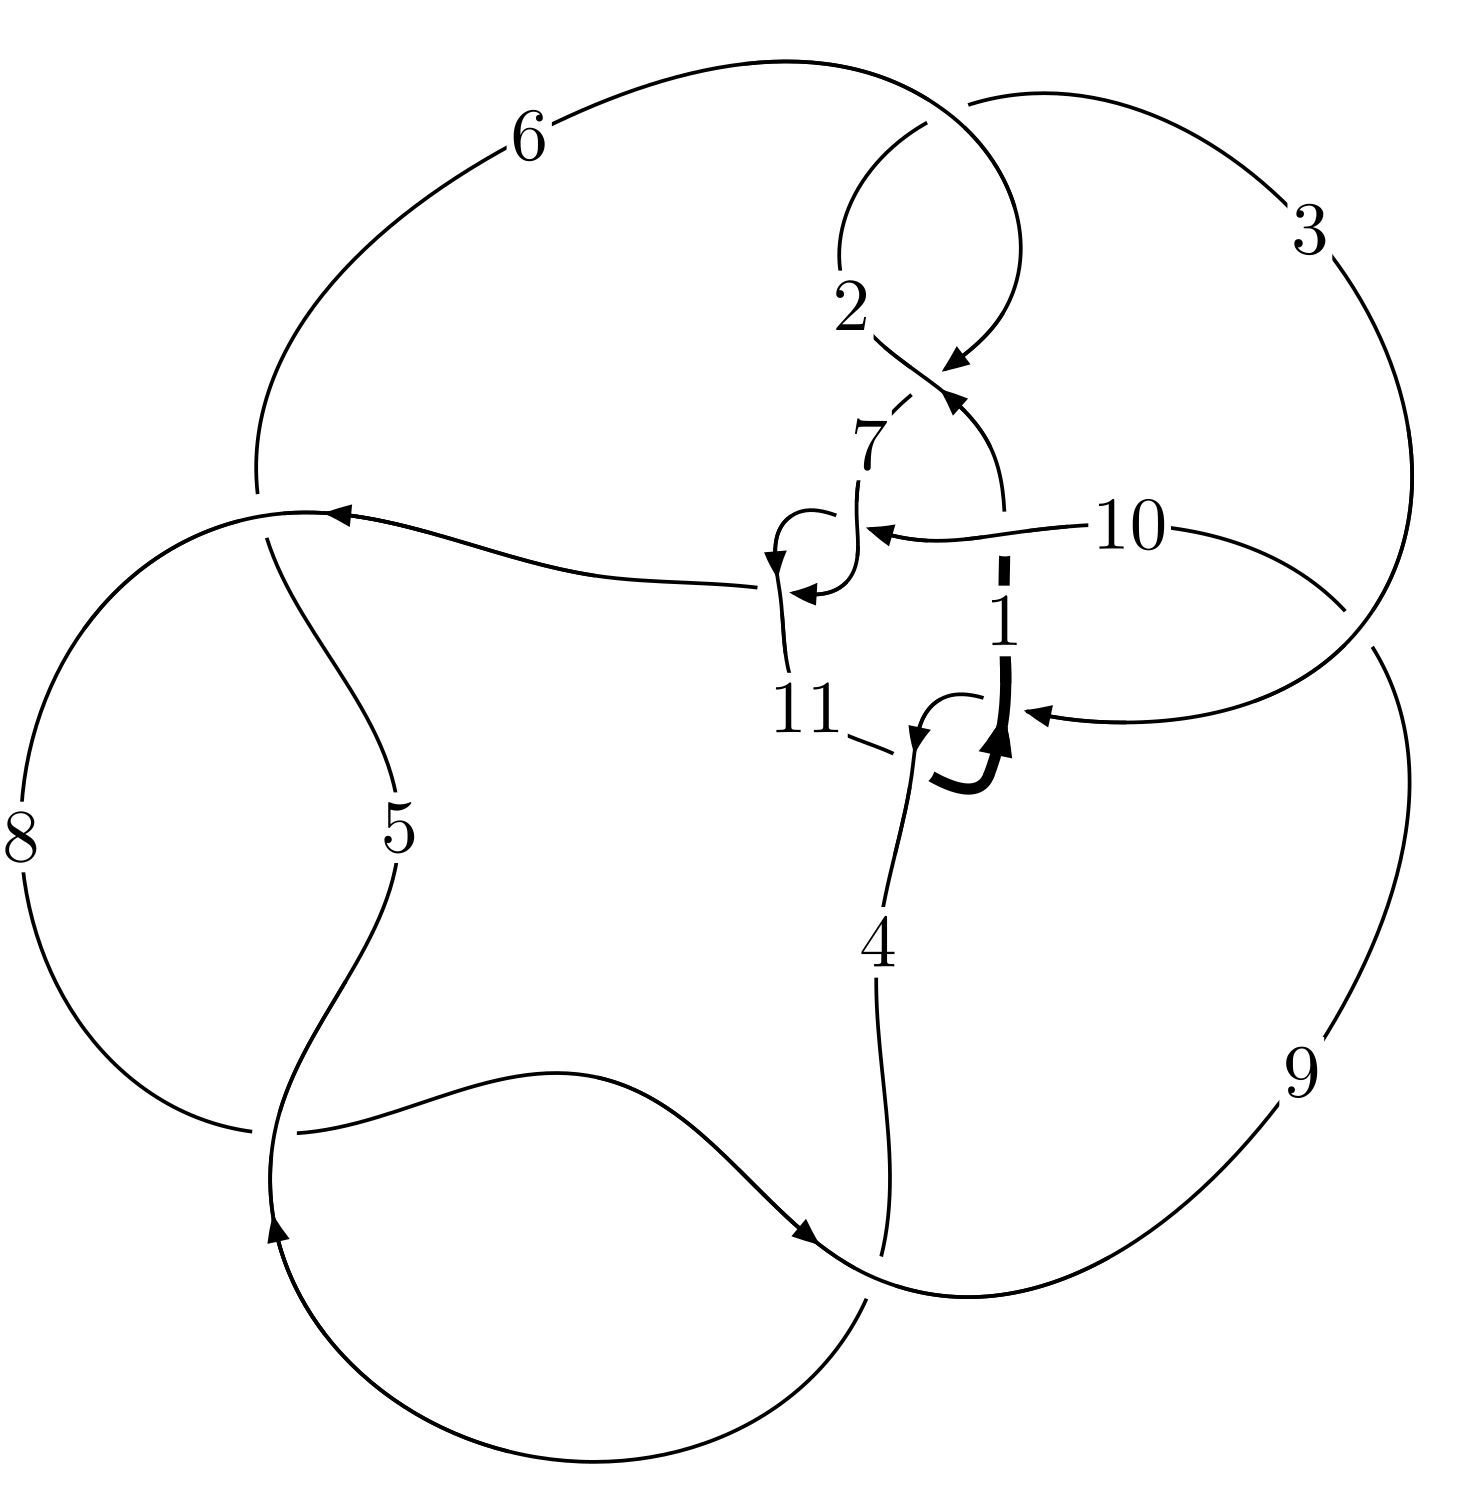
\includegraphics[width=112pt]{../../../GIT/diagram.site/Diagrams/png/580_11a_331.png}\\
\ \ \ A knot diagram\footnotemark}&
\allowdisplaybreaks
\textbf{Linearized knot diagam} \\
\cline{2-2}
 &
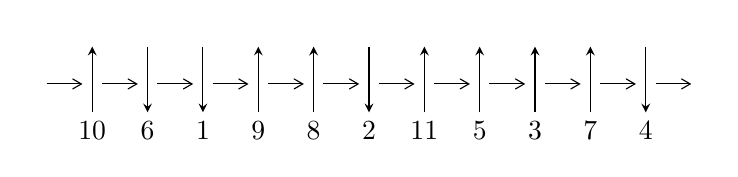
\begin{tikzpicture}[x=20pt, y=17pt]
	% nodes
	\node (C0) at (0, 0) {};
	\node (C1) at (1, 0) {};
	\node (C1U) at (1, +1) {};
	\node (C1D) at (1, -1) {10};

	\node (C2) at (2, 0) {};
	\node (C2U) at (2, +1) {};
	\node (C2D) at (2, -1) {6};

	\node (C3) at (3, 0) {};
	\node (C3U) at (3, +1) {};
	\node (C3D) at (3, -1) {1};

	\node (C4) at (4, 0) {};
	\node (C4U) at (4, +1) {};
	\node (C4D) at (4, -1) {9};

	\node (C5) at (5, 0) {};
	\node (C5U) at (5, +1) {};
	\node (C5D) at (5, -1) {8};

	\node (C6) at (6, 0) {};
	\node (C6U) at (6, +1) {};
	\node (C6D) at (6, -1) {2};

	\node (C7) at (7, 0) {};
	\node (C7U) at (7, +1) {};
	\node (C7D) at (7, -1) {11};

	\node (C8) at (8, 0) {};
	\node (C8U) at (8, +1) {};
	\node (C8D) at (8, -1) {5};

	\node (C9) at (9, 0) {};
	\node (C9U) at (9, +1) {};
	\node (C9D) at (9, -1) {3};

	\node (C10) at (10, 0) {};
	\node (C10U) at (10, +1) {};
	\node (C10D) at (10, -1) {7};

	\node (C11) at (11, 0) {};
	\node (C11U) at (11, +1) {};
	\node (C11D) at (11, -1) {4};
	\node (C12) at (12, 0) {};

	% arrows
	\draw[->,>={angle 60}]
	(C0) edge (C1) (C1) edge (C2) (C2) edge (C3) (C3) edge (C4) (C4) edge (C5) (C5) edge (C6) (C6) edge (C7) (C7) edge (C8) (C8) edge (C9) (C9) edge (C10) (C10) edge (C11) (C11) edge (C12) ;	\draw[->,>=stealth]
	(C1D) edge (C1U) (C2U) edge (C2D) (C3U) edge (C3D) (C4D) edge (C4U) (C5D) edge (C5U) (C6U) edge (C6D) (C7D) edge (C7U) (C8D) edge (C8U) (C9D) edge (C9U) (C10D) edge (C10U) (C11U) edge (C11D) ;
	\end{tikzpicture} \\
\hhline{~~} \\& 
\textbf{Solving Sequence} \\ \cline{2-2} 
 &
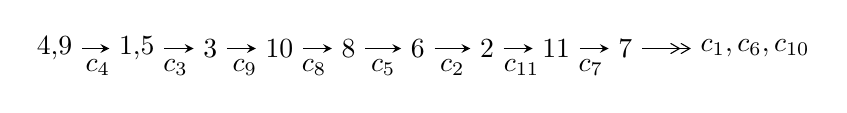
\begin{tikzpicture}[x=25pt, y=7pt]
	% node
	\node (A0) at (-1/8, 0) {4,9};
	\node (A1) at (17/16, 0) {1,5};
	\node (A2) at (17/8, 0) {3};
	\node (A3) at (25/8, 0) {10};
	\node (A4) at (33/8, 0) {8};
	\node (A5) at (41/8, 0) {6};
	\node (A6) at (49/8, 0) {2};
	\node (A7) at (57/8, 0) {11};
	\node (A8) at (65/8, 0) {7};
	\node (C1) at (1/2, -1) {$c_{4}$};
	\node (C2) at (13/8, -1) {$c_{3}$};
	\node (C3) at (21/8, -1) {$c_{9}$};
	\node (C4) at (29/8, -1) {$c_{8}$};
	\node (C5) at (37/8, -1) {$c_{5}$};
	\node (C6) at (45/8, -1) {$c_{2}$};
	\node (C7) at (53/8, -1) {$c_{11}$};
	\node (C8) at (61/8, -1) {$c_{7}$};
	\node (A9) at (10, 0) {$c_{1},c_{6},c_{10}$};

	% edge
	\draw[->,>=stealth]	
	(A0) edge (A1) (A1) edge (A2) (A2) edge (A3) (A3) edge (A4) (A4) edge (A5) (A5) edge (A6) (A6) edge (A7) (A7) edge (A8) ;
	\draw[->>,>={angle 60}]	
	(A8) edge (A9);
\end{tikzpicture} \\ 

\end{tabular} \\

\footnotetext{
The image of knot diagram is generated by the software ``\textbf{Draw programme}" developed by Andrew Bartholomew(\url{http://www.layer8.co.uk/maths/draw/index.htm\#Running-draw}), where we modified some parts for our purpose(\url{https://github.com/CATsTAILs/LinksPainter}).
}\phantom \\ \newline 
\centering \textbf{Ideals for irreducible components\footnotemark of $X_{\text{par}}$} 
 
\begin{align*}
I^u_{1}&=\langle 
8.54894\times10^{95} u^{73}+1.55407\times10^{96} u^{72}+\cdots+2.00526\times10^{96} b-1.27828\times10^{97},\\
\phantom{I^u_{1}}&\phantom{= \langle  }-2.74832\times10^{97} u^{73}-4.48394\times10^{97} u^{72}+\cdots+9.42470\times10^{97} a-1.70641\times10^{99},\\
\phantom{I^u_{1}}&\phantom{= \langle  }u^{74}+3 u^{73}+\cdots+209 u+47\rangle \\
I^u_{2}&=\langle 
u^{15}+3 u^{14}+\cdots+b+2,\;- u^{15}-2 u^{14}+\cdots+a+1,\;u^{17}+2 u^{16}+\cdots+4 u+1\rangle \\
\\
\end{align*}
\raggedright * 2 irreducible components of $\dim_{\mathbb{C}}=0$, with total 91 representations.\\
\footnotetext{All coefficients of polynomials are rational numbers. But the coefficients are sometimes approximated in decimal forms when there is not enough margin.}
\newpage
\renewcommand{\arraystretch}{1}
\centering \section*{I. $I^u_{1}= \langle 8.55\times10^{95} u^{73}+1.55\times10^{96} u^{72}+\cdots+2.01\times10^{96} b-1.28\times10^{97},\;-2.75\times10^{97} u^{73}-4.48\times10^{97} u^{72}+\cdots+9.42\times10^{97} a-1.71\times10^{99},\;u^{74}+3 u^{73}+\cdots+209 u+47 \rangle$}
\flushleft \textbf{(i) Arc colorings}\\
\begin{tabular}{m{7pt} m{180pt} m{7pt} m{180pt} }
\flushright $a_{4}=$&$\begin{pmatrix}1\\0\end{pmatrix}$ \\
\flushright $a_{9}=$&$\begin{pmatrix}0\\u\end{pmatrix}$ \\
\flushright $a_{1}=$&$\begin{pmatrix}0.291608 u^{73}+0.475764 u^{72}+\cdots+26.1433 u+18.1057\\-0.426327 u^{73}-0.774999 u^{72}+\cdots+28.8321 u+6.37465\end{pmatrix}$ \\
\flushright $a_{5}=$&$\begin{pmatrix}1\\- u^2\end{pmatrix}$ \\
\flushright $a_{3}=$&$\begin{pmatrix}0.571268 u^{73}+1.64222 u^{72}+\cdots+103.904 u+29.6284\\-0.233836 u^{73}-0.733389 u^{72}+\cdots-35.5006 u-10.6620\end{pmatrix}$ \\
\flushright $a_{10}=$&$\begin{pmatrix}0.160882 u^{73}+0.784015 u^{72}+\cdots+215.233 u+63.4002\\-0.0885971 u^{73}-1.07134 u^{72}+\cdots-178.043 u-55.1254\end{pmatrix}$ \\
\flushright $a_{8}=$&$\begin{pmatrix}- u\\u^3+u\end{pmatrix}$ \\
\flushright $a_{6}=$&$\begin{pmatrix}u^2+1\\- u^4-2 u^2\end{pmatrix}$ \\
\flushright $a_{2}=$&$\begin{pmatrix}0.756401 u^{73}+2.23671 u^{72}+\cdots+147.047 u+42.9701\\-0.261940 u^{73}-0.983478 u^{72}+\cdots-64.0355 u-19.0821\end{pmatrix}$ \\
\flushright $a_{11}=$&$\begin{pmatrix}-0.134719 u^{73}-0.299235 u^{72}+\cdots+54.9754 u+24.4804\\-0.426327 u^{73}-0.774999 u^{72}+\cdots+28.8321 u+6.37465\end{pmatrix}$ \\
\flushright $a_{7}=$&$\begin{pmatrix}0.303078 u^{73}+0.404458 u^{72}+\cdots-35.9491 u-18.0658\\-0.240564 u^{73}-0.355060 u^{72}+\cdots+2.22918 u-2.45974\end{pmatrix}$\\ \flushright $a_{7}=$&$\begin{pmatrix}0.303078 u^{73}+0.404458 u^{72}+\cdots-35.9491 u-18.0658\\-0.240564 u^{73}-0.355060 u^{72}+\cdots+2.22918 u-2.45974\end{pmatrix}$\\&\end{tabular}
\flushleft \textbf{(ii) Obstruction class $= -1$}\\~\\
\flushleft \textbf{(iii) Cusp Shapes $= -0.681636 u^{73}-3.18822 u^{72}+\cdots-172.342 u-53.5504$}\\~\\
\newpage\renewcommand{\arraystretch}{1}
\flushleft \textbf{(iv) u-Polynomials at the component}\newline \\
\begin{tabular}{m{50pt}|m{274pt}}
Crossings & \hspace{64pt}u-Polynomials at each crossing \\
\hline $$\begin{aligned}c_{1}\end{aligned}$$&$\begin{aligned}
&u^{74}+3 u^{73}+\cdots+59049 u+17047
\end{aligned}$\\
\hline $$\begin{aligned}c_{2},c_{6}\end{aligned}$$&$\begin{aligned}
&u^{74}+2 u^{73}+\cdots-349 u-241
\end{aligned}$\\
\hline $$\begin{aligned}c_{3},c_{11}\end{aligned}$$&$\begin{aligned}
&u^{74}-4 u^{73}+\cdots+578 u-28
\end{aligned}$\\
\hline $$\begin{aligned}c_{4},c_{5},c_{8}\end{aligned}$$&$\begin{aligned}
&u^{74}+3 u^{73}+\cdots+209 u+47
\end{aligned}$\\
\hline $$\begin{aligned}c_{7},c_{10}\end{aligned}$$&$\begin{aligned}
&u^{74}-29 u^{72}+\cdots+4312 u-2881
\end{aligned}$\\
\hline $$\begin{aligned}c_{9}\end{aligned}$$&$\begin{aligned}
&u^{74}- u^{73}+\cdots-2616 u+589
\end{aligned}$\\
\hline
\end{tabular}\\~\\
\newpage\renewcommand{\arraystretch}{1}
\flushleft \textbf{(v) Riley Polynomials at the component}\newline \\
\begin{tabular}{m{50pt}|m{274pt}}
Crossings & \hspace{64pt}Riley Polynomials at each crossing \\
\hline $$\begin{aligned}c_{1}\end{aligned}$$&$\begin{aligned}
&y^{74}-33 y^{73}+\cdots-6606862717 y+290600209
\end{aligned}$\\
\hline $$\begin{aligned}c_{2},c_{6}\end{aligned}$$&$\begin{aligned}
&y^{74}+50 y^{73}+\cdots-32631 y+58081
\end{aligned}$\\
\hline $$\begin{aligned}c_{3},c_{11}\end{aligned}$$&$\begin{aligned}
&y^{74}+46 y^{73}+\cdots-79788 y+784
\end{aligned}$\\
\hline $$\begin{aligned}c_{4},c_{5},c_{8}\end{aligned}$$&$\begin{aligned}
&y^{74}+69 y^{73}+\cdots-23847 y+2209
\end{aligned}$\\
\hline $$\begin{aligned}c_{7},c_{10}\end{aligned}$$&$\begin{aligned}
&y^{74}-58 y^{73}+\cdots-75786956 y+8300161
\end{aligned}$\\
\hline $$\begin{aligned}c_{9}\end{aligned}$$&$\begin{aligned}
&y^{74}-9 y^{73}+\cdots-10759128 y+346921
\end{aligned}$\\
\hline
\end{tabular}\\~\\
\newpage\flushleft \textbf{(vi) Complex Volumes and Cusp Shapes}
$$\begin{array}{c|c|c}  
\text{Solutions to }I^u_{1}& \I (\text{vol} + \sqrt{-1}CS) & \text{Cusp shape}\\
 \hline 
\begin{aligned}
u &= \phantom{-}0.729537 + 0.676863 I \\
a &= \phantom{-}0.868679 + 0.880701 I \\
b &= -0.163050 - 1.175520 I\end{aligned}
 & \phantom{-}4.14808 - 0.48807 I & \phantom{-0.000000 } 0 \\ \hline\begin{aligned}
u &= \phantom{-}0.729537 - 0.676863 I \\
a &= \phantom{-}0.868679 - 0.880701 I \\
b &= -0.163050 + 1.175520 I\end{aligned}
 & \phantom{-}4.14808 + 0.48807 I & \phantom{-0.000000 } 0 \\ \hline\begin{aligned}
u &= -0.977426 + 0.331531 I \\
a &= \phantom{-}0.19408 - 1.78945 I \\
b &= \phantom{-}0.495934 + 1.306620 I\end{aligned}
 & \phantom{-}9.2153 - 11.1163 I & \phantom{-0.000000 } 0 \\ \hline\begin{aligned}
u &= -0.977426 - 0.331531 I \\
a &= \phantom{-}0.19408 + 1.78945 I \\
b &= \phantom{-}0.495934 - 1.306620 I\end{aligned}
 & \phantom{-}9.2153 + 11.1163 I & \phantom{-0.000000 } 0 \\ \hline\begin{aligned}
u &= -0.943528 + 0.160031 I \\
a &= \phantom{-}0.306495 - 1.369660 I \\
b &= -0.498139 + 0.748835 I\end{aligned}
 & \phantom{-}3.11842 + 2.09291 I & \phantom{-0.000000 } 0 \\ \hline\begin{aligned}
u &= -0.943528 - 0.160031 I \\
a &= \phantom{-}0.306495 + 1.369660 I \\
b &= -0.498139 - 0.748835 I\end{aligned}
 & \phantom{-}3.11842 - 2.09291 I & \phantom{-0.000000 } 0 \\ \hline\begin{aligned}
u &= \phantom{-}0.906285 + 0.046309 I \\
a &= \phantom{-}0.37149 + 1.58844 I \\
b &= \phantom{-}0.058387 - 0.883000 I\end{aligned}
 & \phantom{-}2.31155 + 0.31959 I & \phantom{-}6.67473 + 1.17791 I \\ \hline\begin{aligned}
u &= \phantom{-}0.906285 - 0.046309 I \\
a &= \phantom{-}0.37149 - 1.58844 I \\
b &= \phantom{-}0.058387 + 0.883000 I\end{aligned}
 & \phantom{-}2.31155 - 0.31959 I & \phantom{-}6.67473 - 1.17791 I \\ \hline\begin{aligned}
u &= \phantom{-}0.795743 + 0.391782 I \\
a &= -0.33233 - 1.66140 I \\
b &= -0.446696 + 1.338070 I\end{aligned}
 & \phantom{-}4.98505 + 5.49905 I & \phantom{-}7.28766 - 5.67795 I \\ \hline\begin{aligned}
u &= \phantom{-}0.795743 - 0.391782 I \\
a &= -0.33233 + 1.66140 I \\
b &= -0.446696 - 1.338070 I\end{aligned}
 & \phantom{-}4.98505 - 5.49905 I & \phantom{-}7.28766 + 5.67795 I\\
 \hline 
 \end{array}$$\newpage$$\begin{array}{c|c|c}  
\text{Solutions to }I^u_{1}& \I (\text{vol} + \sqrt{-1}CS) & \text{Cusp shape}\\
 \hline 
\begin{aligned}
u &= -0.040289 + 1.123610 I \\
a &= \phantom{-}1.53260 - 0.00979 I \\
b &= \phantom{-}0.755296 - 0.806599 I\end{aligned}
 & \phantom{-}3.32334 + 3.24254 I & \phantom{-0.000000 } 0 \\ \hline\begin{aligned}
u &= -0.040289 - 1.123610 I \\
a &= \phantom{-}1.53260 + 0.00979 I \\
b &= \phantom{-}0.755296 + 0.806599 I\end{aligned}
 & \phantom{-}3.32334 - 3.24254 I & \phantom{-0.000000 } 0 \\ \hline\begin{aligned}
u &= \phantom{-}0.639752 + 0.538004 I \\
a &= -0.48760 - 1.57150 I \\
b &= \phantom{-}0.366420 + 1.022380 I\end{aligned}
 & \phantom{-}3.84856 - 1.30465 I & \phantom{-}7.86722 + 0. I\phantom{ +0.000000I} \\ \hline\begin{aligned}
u &= \phantom{-}0.639752 - 0.538004 I \\
a &= -0.48760 + 1.57150 I \\
b &= \phantom{-}0.366420 - 1.022380 I\end{aligned}
 & \phantom{-}3.84856 + 1.30465 I & \phantom{-}7.86722 + 0. I\phantom{ +0.000000I} \\ \hline\begin{aligned}
u &= \phantom{-}0.000251 + 1.184520 I \\
a &= -1.98927 - 1.08115 I \\
b &= -0.096365 + 0.840334 I\end{aligned}
 & \phantom{-}2.78997 - 3.49775 I & \phantom{-0.000000 } 0 \\ \hline\begin{aligned}
u &= \phantom{-}0.000251 - 1.184520 I \\
a &= -1.98927 + 1.08115 I \\
b &= -0.096365 - 0.840334 I\end{aligned}
 & \phantom{-}2.78997 + 3.49775 I & \phantom{-0.000000 } 0 \\ \hline\begin{aligned}
u &= -0.159658 + 1.194760 I \\
a &= -0.089269 + 0.550066 I \\
b &= \phantom{-}0.29274 - 1.69325 I\end{aligned}
 & \phantom{-}6.20327 - 3.01035 I & \phantom{-0.000000 } 0 \\ \hline\begin{aligned}
u &= -0.159658 - 1.194760 I \\
a &= -0.089269 - 0.550066 I \\
b &= \phantom{-}0.29274 + 1.69325 I\end{aligned}
 & \phantom{-}6.20327 + 3.01035 I & \phantom{-0.000000 } 0 \\ \hline\begin{aligned}
u &= -0.546934 + 0.540048 I \\
a &= -0.27605 - 1.72599 I \\
b &= \phantom{-}0.276972 + 0.159839 I\end{aligned}
 & \phantom{-}4.14609 + 2.20221 I & \phantom{-}4.65992 + 1.32874 I \\ \hline\begin{aligned}
u &= -0.546934 - 0.540048 I \\
a &= -0.27605 + 1.72599 I \\
b &= \phantom{-}0.276972 - 0.159839 I\end{aligned}
 & \phantom{-}4.14609 - 2.20221 I & \phantom{-}4.65992 - 1.32874 I\\
 \hline 
 \end{array}$$\newpage$$\begin{array}{c|c|c}  
\text{Solutions to }I^u_{1}& \I (\text{vol} + \sqrt{-1}CS) & \text{Cusp shape}\\
 \hline 
\begin{aligned}
u &= -0.107310 + 1.251050 I \\
a &= \phantom{-}0.06868 - 1.71275 I \\
b &= -0.03954 + 1.50942 I\end{aligned}
 & \phantom{-}5.33288 + 0.16111 I & \phantom{-0.000000 } 0 \\ \hline\begin{aligned}
u &= -0.107310 - 1.251050 I \\
a &= \phantom{-}0.06868 + 1.71275 I \\
b &= -0.03954 - 1.50942 I\end{aligned}
 & \phantom{-}5.33288 - 0.16111 I & \phantom{-0.000000 } 0 \\ \hline\begin{aligned}
u &= \phantom{-}0.643915 + 0.344718 I \\
a &= \phantom{-}0.68185 + 2.68762 I \\
b &= \phantom{-}0.339896 - 1.158020 I\end{aligned}
 & \phantom{-}4.28355 + 5.31590 I & \phantom{-}8.32121 - 6.98455 I \\ \hline\begin{aligned}
u &= \phantom{-}0.643915 - 0.344718 I \\
a &= \phantom{-}0.68185 - 2.68762 I \\
b &= \phantom{-}0.339896 + 1.158020 I\end{aligned}
 & \phantom{-}4.28355 - 5.31590 I & \phantom{-}8.32121 + 6.98455 I \\ \hline\begin{aligned}
u &= -0.672302 + 0.275487 I \\
a &= -0.463214 + 0.218192 I \\
b &= \phantom{-}0.994473 + 0.038479 I\end{aligned}
 & \phantom{-}5.09446 - 5.88932 I & \phantom{-}7.14918 + 5.98042 I \\ \hline\begin{aligned}
u &= -0.672302 - 0.275487 I \\
a &= -0.463214 - 0.218192 I \\
b &= \phantom{-}0.994473 - 0.038479 I\end{aligned}
 & \phantom{-}5.09446 + 5.88932 I & \phantom{-}7.14918 - 5.98042 I \\ \hline\begin{aligned}
u &= \phantom{-}0.534184 + 0.471782 I \\
a &= -0.203180 + 0.429819 I \\
b &= \phantom{-}0.568753 + 0.043415 I\end{aligned}
 & \phantom{-}1.09531 + 1.83562 I & \phantom{-}2.55599 - 4.19616 I \\ \hline\begin{aligned}
u &= \phantom{-}0.534184 - 0.471782 I \\
a &= -0.203180 - 0.429819 I \\
b &= \phantom{-}0.568753 - 0.043415 I\end{aligned}
 & \phantom{-}1.09531 - 1.83562 I & \phantom{-}2.55599 + 4.19616 I \\ \hline\begin{aligned}
u &= -0.781242 + 1.028170 I \\
a &= -0.589220 + 0.832021 I \\
b &= \phantom{-}0.342776 - 1.173760 I\end{aligned}
 & \phantom{-}7.24129 + 5.12075 I & \phantom{-0.000000 } 0 \\ \hline\begin{aligned}
u &= -0.781242 - 1.028170 I \\
a &= -0.589220 - 0.832021 I \\
b &= \phantom{-}0.342776 + 1.173760 I\end{aligned}
 & \phantom{-}7.24129 - 5.12075 I & \phantom{-0.000000 } 0\\
 \hline 
 \end{array}$$\newpage$$\begin{array}{c|c|c}  
\text{Solutions to }I^u_{1}& \I (\text{vol} + \sqrt{-1}CS) & \text{Cusp shape}\\
 \hline 
\begin{aligned}
u &= \phantom{-}0.162659 + 1.334780 I \\
a &= -0.513861 - 0.136702 I \\
b &= -1.40639 - 0.48404 I\end{aligned}
 & -4.07205 + 2.16735 I & \phantom{-0.000000 } 0 \\ \hline\begin{aligned}
u &= \phantom{-}0.162659 - 1.334780 I \\
a &= -0.513861 + 0.136702 I \\
b &= -1.40639 + 0.48404 I\end{aligned}
 & -4.07205 - 2.16735 I & \phantom{-0.000000 } 0 \\ \hline\begin{aligned}
u &= -0.077830 + 1.356390 I \\
a &= \phantom{-}0.719009 - 0.826751 I \\
b &= \phantom{-}0.343236 + 0.909674 I\end{aligned}
 & -2.84114 + 0.89469 I & \phantom{-0.000000 } 0 \\ \hline\begin{aligned}
u &= -0.077830 - 1.356390 I \\
a &= \phantom{-}0.719009 + 0.826751 I \\
b &= \phantom{-}0.343236 - 0.909674 I\end{aligned}
 & -2.84114 - 0.89469 I & \phantom{-0.000000 } 0 \\ \hline\begin{aligned}
u &= -0.173008 + 1.356910 I \\
a &= -1.01178 + 1.02451 I \\
b &= -0.593612 - 1.233660 I\end{aligned}
 & -3.89386 - 4.74590 I & \phantom{-0.000000 } 0 \\ \hline\begin{aligned}
u &= -0.173008 - 1.356910 I \\
a &= -1.01178 - 1.02451 I \\
b &= -0.593612 + 1.233660 I\end{aligned}
 & -3.89386 + 4.74590 I & \phantom{-0.000000 } 0 \\ \hline\begin{aligned}
u &= -0.605325 + 0.154014 I \\
a &= \phantom{-}0.73564 - 1.74796 I \\
b &= \phantom{-}0.50294 + 1.38892 I\end{aligned}
 & \phantom{-}9.24632 + 0.28330 I & \phantom{-}12.69819 + 0.63805 I \\ \hline\begin{aligned}
u &= -0.605325 - 0.154014 I \\
a &= \phantom{-}0.73564 + 1.74796 I \\
b &= \phantom{-}0.50294 - 1.38892 I\end{aligned}
 & \phantom{-}9.24632 - 0.28330 I & \phantom{-}12.69819 - 0.63805 I \\ \hline\begin{aligned}
u &= -0.243787 + 1.360410 I \\
a &= \phantom{-}1.128220 - 0.271966 I \\
b &= \phantom{-}0.755260 + 1.157050 I\end{aligned}
 & \phantom{-}4.42124 - 2.83103 I & \phantom{-0.000000 } 0 \\ \hline\begin{aligned}
u &= -0.243787 - 1.360410 I \\
a &= \phantom{-}1.128220 + 0.271966 I \\
b &= \phantom{-}0.755260 - 1.157050 I\end{aligned}
 & \phantom{-}4.42124 + 2.83103 I & \phantom{-0.000000 } 0\\
 \hline 
 \end{array}$$\newpage$$\begin{array}{c|c|c}  
\text{Solutions to }I^u_{1}& \I (\text{vol} + \sqrt{-1}CS) & \text{Cusp shape}\\
 \hline 
\begin{aligned}
u &= \phantom{-}0.327994 + 1.351610 I \\
a &= -0.439710 - 1.149670 I \\
b &= -0.290077 + 1.121430 I\end{aligned}
 & -2.02174 + 4.04028 I & \phantom{-0.000000 } 0 \\ \hline\begin{aligned}
u &= \phantom{-}0.327994 - 1.351610 I \\
a &= -0.439710 + 1.149670 I \\
b &= -0.290077 - 1.121430 I\end{aligned}
 & -2.02174 - 4.04028 I & \phantom{-0.000000 } 0 \\ \hline\begin{aligned}
u &= -0.195271 + 1.386520 I \\
a &= -1.62301 - 0.11159 I \\
b &= -0.143149 - 1.028900 I\end{aligned}
 & \phantom{-}3.52909 - 4.64112 I & \phantom{-0.000000 } 0 \\ \hline\begin{aligned}
u &= -0.195271 - 1.386520 I \\
a &= -1.62301 + 0.11159 I \\
b &= -0.143149 + 1.028900 I\end{aligned}
 & \phantom{-}3.52909 + 4.64112 I & \phantom{-0.000000 } 0 \\ \hline\begin{aligned}
u &= -0.47948 + 1.33348 I \\
a &= -0.76428 + 1.24106 I \\
b &= -0.600996 - 0.993957 I\end{aligned}
 & -0.64736 - 7.35044 I & \phantom{-0.000000 } 0 \\ \hline\begin{aligned}
u &= -0.47948 - 1.33348 I \\
a &= -0.76428 - 1.24106 I \\
b &= -0.600996 + 0.993957 I\end{aligned}
 & -0.64736 + 7.35044 I & \phantom{-0.000000 } 0 \\ \hline\begin{aligned}
u &= -0.00514 + 1.42211 I \\
a &= -0.340891 + 0.208274 I \\
b &= -0.964892 + 0.318084 I\end{aligned}
 & -6.82153 + 0.92955 I & \phantom{-0.000000 } 0 \\ \hline\begin{aligned}
u &= -0.00514 - 1.42211 I \\
a &= -0.340891 - 0.208274 I \\
b &= -0.964892 - 0.318084 I\end{aligned}
 & -6.82153 - 0.92955 I & \phantom{-0.000000 } 0 \\ \hline\begin{aligned}
u &= -0.30682 + 1.39309 I \\
a &= \phantom{-}0.0331436 - 0.1004190 I \\
b &= -0.778543 + 0.548393 I\end{aligned}
 & -1.97320 - 2.18673 I & \phantom{-0.000000 } 0 \\ \hline\begin{aligned}
u &= -0.30682 - 1.39309 I \\
a &= \phantom{-}0.0331436 + 0.1004190 I \\
b &= -0.778543 - 0.548393 I\end{aligned}
 & -1.97320 + 2.18673 I & \phantom{-0.000000 } 0\\
 \hline 
 \end{array}$$\newpage$$\begin{array}{c|c|c}  
\text{Solutions to }I^u_{1}& \I (\text{vol} + \sqrt{-1}CS) & \text{Cusp shape}\\
 \hline 
\begin{aligned}
u &= -0.26985 + 1.40575 I \\
a &= \phantom{-}0.280548 - 0.298110 I \\
b &= \phantom{-}1.265840 - 0.184891 I\end{aligned}
 & -0.26002 - 9.34220 I & \phantom{-0.000000 } 0 \\ \hline\begin{aligned}
u &= -0.26985 - 1.40575 I \\
a &= \phantom{-}0.280548 + 0.298110 I \\
b &= \phantom{-}1.265840 + 0.184891 I\end{aligned}
 & -0.26002 + 9.34220 I & \phantom{-0.000000 } 0 \\ \hline\begin{aligned}
u &= \phantom{-}0.25598 + 1.42903 I \\
a &= \phantom{-}1.10171 + 1.29179 I \\
b &= \phantom{-}0.429957 - 1.299690 I\end{aligned}
 & -1.37538 + 8.63536 I & \phantom{-0.000000 } 0 \\ \hline\begin{aligned}
u &= \phantom{-}0.25598 - 1.42903 I \\
a &= \phantom{-}1.10171 - 1.29179 I \\
b &= \phantom{-}0.429957 + 1.299690 I\end{aligned}
 & -1.37538 - 8.63536 I & \phantom{-0.000000 } 0 \\ \hline\begin{aligned}
u &= \phantom{-}0.09320 + 1.45012 I \\
a &= \phantom{-}0.367361 - 0.401509 I \\
b &= \phantom{-}0.570488 + 0.736664 I\end{aligned}
 & -3.23957 + 0.97155 I & \phantom{-0.000000 } 0 \\ \hline\begin{aligned}
u &= \phantom{-}0.09320 - 1.45012 I \\
a &= \phantom{-}0.367361 + 0.401509 I \\
b &= \phantom{-}0.570488 - 0.736664 I\end{aligned}
 & -3.23957 - 0.97155 I & \phantom{-0.000000 } 0 \\ \hline\begin{aligned}
u &= \phantom{-}0.33909 + 1.42618 I \\
a &= \phantom{-}0.897474 + 0.790587 I \\
b &= \phantom{-}0.412854 - 0.931526 I\end{aligned}
 & -2.65219 + 4.84548 I & \phantom{-0.000000 } 0 \\ \hline\begin{aligned}
u &= \phantom{-}0.33909 - 1.42618 I \\
a &= \phantom{-}0.897474 - 0.790587 I \\
b &= \phantom{-}0.412854 + 0.931526 I\end{aligned}
 & -2.65219 - 4.84548 I & \phantom{-0.000000 } 0 \\ \hline\begin{aligned}
u &= \phantom{-}0.14497 + 1.48045 I \\
a &= \phantom{-}0.308110 + 0.341335 I \\
b &= \phantom{-}0.732906 + 0.027438 I\end{aligned}
 & -5.30403 + 4.22277 I & \phantom{-0.000000 } 0 \\ \hline\begin{aligned}
u &= \phantom{-}0.14497 - 1.48045 I \\
a &= \phantom{-}0.308110 - 0.341335 I \\
b &= \phantom{-}0.732906 - 0.027438 I\end{aligned}
 & -5.30403 - 4.22277 I & \phantom{-0.000000 } 0\\
 \hline 
 \end{array}$$\newpage$$\begin{array}{c|c|c}  
\text{Solutions to }I^u_{1}& \I (\text{vol} + \sqrt{-1}CS) & \text{Cusp shape}\\
 \hline 
\begin{aligned}
u &= -0.480633 + 0.177328 I \\
a &= -2.91872 + 1.85536 I \\
b &= -0.012937 - 1.270620 I\end{aligned}
 & \phantom{-}8.59018 - 2.10885 I & \phantom{-}14.2741 + 3.7354 I \\ \hline\begin{aligned}
u &= -0.480633 - 0.177328 I \\
a &= -2.91872 - 1.85536 I \\
b &= -0.012937 + 1.270620 I\end{aligned}
 & \phantom{-}8.59018 + 2.10885 I & \phantom{-}14.2741 - 3.7354 I \\ \hline\begin{aligned}
u &= \phantom{-}0.31043 + 1.46205 I \\
a &= -0.917093 - 0.764806 I \\
b &= -0.70775 + 1.34146 I\end{aligned}
 & -0.93880 + 9.51927 I & \phantom{-0.000000 } 0 \\ \hline\begin{aligned}
u &= \phantom{-}0.31043 - 1.46205 I \\
a &= -0.917093 + 0.764806 I \\
b &= -0.70775 - 1.34146 I\end{aligned}
 & -0.93880 - 9.51927 I & \phantom{-0.000000 } 0 \\ \hline\begin{aligned}
u &= -0.38759 + 1.47330 I \\
a &= \phantom{-}0.98510 - 1.03601 I \\
b &= \phantom{-}0.64917 + 1.35397 I\end{aligned}
 & \phantom{-}3.4628 - 16.0068 I & \phantom{-0.000000 } 0 \\ \hline\begin{aligned}
u &= -0.38759 - 1.47330 I \\
a &= \phantom{-}0.98510 + 1.03601 I \\
b &= \phantom{-}0.64917 - 1.35397 I\end{aligned}
 & \phantom{-}3.4628 + 16.0068 I & \phantom{-0.000000 } 0 \\ \hline\begin{aligned}
u &= -0.463049 + 0.111626 I \\
a &= \phantom{-}0.09477 + 2.83159 I \\
b &= -0.354673 - 1.019580 I\end{aligned}
 & \phantom{-}0.80708 - 2.42495 I & \phantom{-}0.09499 + 4.46298 I \\ \hline\begin{aligned}
u &= -0.463049 - 0.111626 I \\
a &= \phantom{-}0.09477 - 2.83159 I \\
b &= -0.354673 + 1.019580 I\end{aligned}
 & \phantom{-}0.80708 + 2.42495 I & \phantom{-}0.09499 - 4.46298 I \\ \hline\begin{aligned}
u &= \phantom{-}0.437958\phantom{ +0.000000I} \\
a &= \phantom{-}0.177670\phantom{ +0.000000I} \\
b &= -1.22248\phantom{ +0.000000I}\end{aligned}
 & \phantom{-}0.260961\phantom{ +0.000000I} & \phantom{-}17.7580\phantom{ +0.000000I} \\ \hline\begin{aligned}
u &= -0.024389 + 0.433644 I \\
a &= \phantom{-}0.483657 + 0.315936 I \\
b &= -0.542238 + 0.411060 I\end{aligned}
 & -0.93889 + 1.06996 I & -3.82834 - 4.75783 I\\
 \hline 
 \end{array}$$\newpage$$\begin{array}{c|c|c}  
\text{Solutions to }I^u_{1}& \I (\text{vol} + \sqrt{-1}CS) & \text{Cusp shape}\\
 \hline 
\begin{aligned}
u &= -0.024389 - 0.433644 I \\
a &= \phantom{-}0.483657 - 0.315936 I \\
b &= -0.542238 - 0.411060 I\end{aligned}
 & -0.93889 - 1.06996 I & -3.82834 + 4.75783 I \\ \hline\begin{aligned}
u &= \phantom{-}0.413553\phantom{ +0.000000I} \\
a &= \phantom{-}1.39372\phantom{ +0.000000I} \\
b &= \phantom{-}0.0976025\phantom{ +0.000000I}\end{aligned}
 & \phantom{-}1.01618\phantom{ +0.000000I} & \phantom{-}11.7030\phantom{ +0.000000I} \\ \hline\begin{aligned}
u &= \phantom{-}0.13112 + 1.67227 I \\
a &= \phantom{-}0.249215 + 0.136146 I \\
b &= \phantom{-}0.047190 - 0.821814 I\end{aligned}
 & -4.10246 + 2.99543 I & \phantom{-0.000000 } 0 \\ \hline\begin{aligned}
u &= \phantom{-}0.13112 - 1.67227 I \\
a &= \phantom{-}0.249215 - 0.136146 I \\
b &= \phantom{-}0.047190 + 0.821814 I\end{aligned}
 & -4.10246 - 2.99543 I & \phantom{-0.000000 } 0\\
 \hline 
 \end{array}$$\newpage\newpage\renewcommand{\arraystretch}{1}
\centering \section*{II. $I^u_{2}= \langle u^{15}+3 u^{14}+\cdots+b+2,\;- u^{15}-2 u^{14}+\cdots+a+1,\;u^{17}+2 u^{16}+\cdots+4 u+1 \rangle$}
\flushleft \textbf{(i) Arc colorings}\\
\begin{tabular}{m{7pt} m{180pt} m{7pt} m{180pt} }
\flushright $a_{4}=$&$\begin{pmatrix}1\\0\end{pmatrix}$ \\
\flushright $a_{9}=$&$\begin{pmatrix}0\\u\end{pmatrix}$ \\
\flushright $a_{1}=$&$\begin{pmatrix}u^{15}+2 u^{14}+\cdots+2 u-1\\- u^{15}-3 u^{14}+\cdots-6 u-2\end{pmatrix}$ \\
\flushright $a_{5}=$&$\begin{pmatrix}1\\- u^2\end{pmatrix}$ \\
\flushright $a_{3}=$&$\begin{pmatrix}-2 u^{16}-4 u^{15}+\cdots-12 u^2- u\\2 u^{15}+3 u^{14}+\cdots+6 u+1\end{pmatrix}$ \\
\flushright $a_{10}=$&$\begin{pmatrix}- u^{16}-3 u^{15}+\cdots-7 u^2- u\\3 u^{15}+6 u^{14}+\cdots+14 u+3\end{pmatrix}$ \\
\flushright $a_{8}=$&$\begin{pmatrix}- u\\u^3+u\end{pmatrix}$ \\
\flushright $a_{6}=$&$\begin{pmatrix}u^2+1\\- u^4-2 u^2\end{pmatrix}$ \\
\flushright $a_{2}=$&$\begin{pmatrix}-2 u^{16}-3 u^{15}+\cdots-10 u^2+3 u\\u^{15}+u^{14}+\cdots+6 u+1\end{pmatrix}$ \\
\flushright $a_{11}=$&$\begin{pmatrix}- u^{14}-2 u^{13}+\cdots-4 u-3\\- u^{15}-3 u^{14}+\cdots-6 u-2\end{pmatrix}$ \\
\flushright $a_{7}=$&$\begin{pmatrix}u^{16}+3 u^{15}+\cdots+8 u+4\\u^{16}+u^{15}+\cdots+4 u+1\end{pmatrix}$\\ \flushright $a_{7}=$&$\begin{pmatrix}u^{16}+3 u^{15}+\cdots+8 u+4\\u^{16}+u^{15}+\cdots+4 u+1\end{pmatrix}$\\&\end{tabular}
\flushleft \textbf{(ii) Obstruction class $= 1$}\\~\\
\flushleft \textbf{(iii) Cusp Shapes $= - u^{16}+u^{15}-9 u^{14}+3 u^{13}-38 u^{12}-17 u^{11}-90 u^{10}-94 u^9-121 u^8-168 u^7-101 u^6-123 u^5-74 u^4-22 u^3-43 u^2+4 u$}\\~\\
\newpage\renewcommand{\arraystretch}{1}
\flushleft \textbf{(iv) u-Polynomials at the component}\newline \\
\begin{tabular}{m{50pt}|m{274pt}}
Crossings & \hspace{64pt}u-Polynomials at each crossing \\
\hline $$\begin{aligned}c_{1}\end{aligned}$$&$\begin{aligned}
&u^{17}-6 u^{16}+\cdots+6 u-1
\end{aligned}$\\
\hline $$\begin{aligned}c_{2}\end{aligned}$$&$\begin{aligned}
&u^{17}+u^{16}+\cdots-5 u^2-1
\end{aligned}$\\
\hline $$\begin{aligned}c_{3}\end{aligned}$$&$\begin{aligned}
&u^{17}+3 u^{16}+\cdots+3 u+1
\end{aligned}$\\
\hline $$\begin{aligned}c_{4},c_{5}\end{aligned}$$&$\begin{aligned}
&u^{17}+2 u^{16}+\cdots+4 u+1
\end{aligned}$\\
\hline $$\begin{aligned}c_{6}\end{aligned}$$&$\begin{aligned}
&u^{17}- u^{16}+\cdots+5 u^2+1
\end{aligned}$\\
\hline $$\begin{aligned}c_{7}\end{aligned}$$&$\begin{aligned}
&u^{17}-3 u^{16}+\cdots- u+1
\end{aligned}$\\
\hline $$\begin{aligned}c_{8}\end{aligned}$$&$\begin{aligned}
&u^{17}-2 u^{16}+\cdots+4 u-1
\end{aligned}$\\
\hline $$\begin{aligned}c_{9}\end{aligned}$$&$\begin{aligned}
&u^{17}-8 u^{14}+\cdots+9 u+1
\end{aligned}$\\
\hline $$\begin{aligned}c_{10}\end{aligned}$$&$\begin{aligned}
&u^{17}+3 u^{16}+\cdots- u-1
\end{aligned}$\\
\hline $$\begin{aligned}c_{11}\end{aligned}$$&$\begin{aligned}
&u^{17}-3 u^{16}+\cdots+3 u-1
\end{aligned}$\\
\hline
\end{tabular}\\~\\
\newpage\renewcommand{\arraystretch}{1}
\flushleft \textbf{(v) Riley Polynomials at the component}\newline \\
\begin{tabular}{m{50pt}|m{274pt}}
Crossings & \hspace{64pt}Riley Polynomials at each crossing \\
\hline $$\begin{aligned}c_{1}\end{aligned}$$&$\begin{aligned}
&y^{17}-4 y^{16}+\cdots+12 y-1
\end{aligned}$\\
\hline $$\begin{aligned}c_{2},c_{6}\end{aligned}$$&$\begin{aligned}
&y^{17}+11 y^{16}+\cdots-10 y-1
\end{aligned}$\\
\hline $$\begin{aligned}c_{3},c_{11}\end{aligned}$$&$\begin{aligned}
&y^{17}+11 y^{16}+\cdots-11 y-1
\end{aligned}$\\
\hline $$\begin{aligned}c_{4},c_{5},c_{8}\end{aligned}$$&$\begin{aligned}
&y^{17}+18 y^{16}+\cdots+6 y-1
\end{aligned}$\\
\hline $$\begin{aligned}c_{7},c_{10}\end{aligned}$$&$\begin{aligned}
&y^{17}-17 y^{16}+\cdots+15 y-1
\end{aligned}$\\
\hline $$\begin{aligned}c_{9}\end{aligned}$$&$\begin{aligned}
&y^{17}-12 y^{14}+\cdots+55 y-1
\end{aligned}$\\
\hline
\end{tabular}\\~\\
\newpage\flushleft \textbf{(vi) Complex Volumes and Cusp Shapes}
$$\begin{array}{c|c|c}  
\text{Solutions to }I^u_{2}& \I (\text{vol} + \sqrt{-1}CS) & \text{Cusp shape}\\
 \hline 
\begin{aligned}
u &= -0.917169 + 0.197212 I \\
a &= \phantom{-}0.33537 - 1.51249 I \\
b &= -0.325330 + 0.891594 I\end{aligned}
 & \phantom{-}1.91049 + 1.40877 I & \phantom{-}1.99755 - 3.08552 I \\ \hline\begin{aligned}
u &= -0.917169 - 0.197212 I \\
a &= \phantom{-}0.33537 + 1.51249 I \\
b &= -0.325330 - 0.891594 I\end{aligned}
 & \phantom{-}1.91049 - 1.40877 I & \phantom{-}1.99755 + 3.08552 I \\ \hline\begin{aligned}
u &= \phantom{-}0.035271 + 1.235610 I \\
a &= \phantom{-}0.70102 - 1.33099 I \\
b &= \phantom{-}0.19425 + 1.50294 I\end{aligned}
 & \phantom{-}5.20161 + 1.70001 I & \phantom{-}5.37273 - 2.73061 I \\ \hline\begin{aligned}
u &= \phantom{-}0.035271 - 1.235610 I \\
a &= \phantom{-}0.70102 + 1.33099 I \\
b &= \phantom{-}0.19425 - 1.50294 I\end{aligned}
 & \phantom{-}5.20161 - 1.70001 I & \phantom{-}5.37273 + 2.73061 I \\ \hline\begin{aligned}
u &= \phantom{-}0.171164 + 1.296500 I \\
a &= \phantom{-}1.75533 - 0.00516 I \\
b &= \phantom{-}0.459524 - 0.755278 I\end{aligned}
 & \phantom{-}2.00726 + 4.91579 I & \phantom{-}2.45525 - 6.27876 I \\ \hline\begin{aligned}
u &= \phantom{-}0.171164 - 1.296500 I \\
a &= \phantom{-}1.75533 + 0.00516 I \\
b &= \phantom{-}0.459524 + 0.755278 I\end{aligned}
 & \phantom{-}2.00726 - 4.91579 I & \phantom{-}2.45525 + 6.27876 I \\ \hline\begin{aligned}
u &= \phantom{-}0.409969 + 0.519303 I \\
a &= -1.08154 - 2.81632 I \\
b &= \phantom{-}0.226258 + 0.744134 I\end{aligned}
 & \phantom{-}4.98146 - 2.80089 I & \phantom{-}12.23664 + 2.91381 I \\ \hline\begin{aligned}
u &= \phantom{-}0.409969 - 0.519303 I \\
a &= -1.08154 + 2.81632 I \\
b &= \phantom{-}0.226258 - 0.744134 I\end{aligned}
 & \phantom{-}4.98146 + 2.80089 I & \phantom{-}12.23664 - 2.91381 I \\ \hline\begin{aligned}
u &= \phantom{-}0.089248 + 0.610949 I \\
a &= -0.658805 - 0.382206 I \\
b &= \phantom{-}0.101471 - 1.352370 I\end{aligned}
 & \phantom{-}7.59288 - 1.25507 I & \phantom{-}8.41084 + 0.24395 I \\ \hline\begin{aligned}
u &= \phantom{-}0.089248 - 0.610949 I \\
a &= -0.658805 + 0.382206 I \\
b &= \phantom{-}0.101471 + 1.352370 I\end{aligned}
 & \phantom{-}7.59288 + 1.25507 I & \phantom{-}8.41084 - 0.24395 I\\
 \hline 
 \end{array}$$\newpage$$\begin{array}{c|c|c}  
\text{Solutions to }I^u_{2}& \I (\text{vol} + \sqrt{-1}CS) & \text{Cusp shape}\\
 \hline 
\begin{aligned}
u &= -0.124683 + 1.379790 I \\
a &= -0.427475 - 0.148819 I \\
b &= -1.044610 + 0.361468 I\end{aligned}
 & -4.85490 - 1.43958 I & -1.090547 - 0.048277 I \\ \hline\begin{aligned}
u &= -0.124683 - 1.379790 I \\
a &= -0.427475 + 0.148819 I \\
b &= -1.044610 - 0.361468 I\end{aligned}
 & -4.85490 + 1.43958 I & -1.090547 + 0.048277 I \\ \hline\begin{aligned}
u &= -0.36245 + 1.38049 I \\
a &= -0.841748 + 1.085670 I \\
b &= -0.467784 - 1.122320 I\end{aligned}
 & -2.18873 - 6.08260 I & \phantom{-}3.68269 + 6.06370 I \\ \hline\begin{aligned}
u &= -0.36245 - 1.38049 I \\
a &= -0.841748 - 1.085670 I \\
b &= -0.467784 + 1.122320 I\end{aligned}
 & -2.18873 + 6.08260 I & \phantom{-}3.68269 - 6.06370 I \\ \hline\begin{aligned}
u &= -0.17262 + 1.59957 I \\
a &= \phantom{-}0.019317 - 0.357002 I \\
b &= -0.175891 + 0.545807 I\end{aligned}
 & -4.71707 - 2.60778 I & -2.21051 - 0.39909 I \\ \hline\begin{aligned}
u &= -0.17262 - 1.59957 I \\
a &= \phantom{-}0.019317 + 0.357002 I \\
b &= -0.175891 - 0.545807 I\end{aligned}
 & -4.71707 + 2.60778 I & -2.21051 + 0.39909 I \\ \hline\begin{aligned}
u &= -0.257452\phantom{ +0.000000I} \\
a &= -1.60294\phantom{ +0.000000I} \\
b &= -0.935779\phantom{ +0.000000I}\end{aligned}
 & -0.126778\phantom{ +0.000000I} & -3.70930\phantom{ +0.000000I}\\
 \hline 
 \end{array}$$\newpage
\newpage\renewcommand{\arraystretch}{1}
\centering \section*{ III. u-Polynomials}
\begin{tabular}{m{50pt}|m{274pt}}
Crossings & \hspace{64pt}u-Polynomials at each crossing \\
\hline $$\begin{aligned}c_{1}\end{aligned}$$&$\begin{aligned}
&(u^{17}-6 u^{16}+\cdots+6 u-1)(u^{74}+3 u^{73}+\cdots+59049 u+17047)
\end{aligned}$\\
\hline $$\begin{aligned}c_{2}\end{aligned}$$&$\begin{aligned}
&(u^{17}+u^{16}+\cdots-5 u^2-1)(u^{74}+2 u^{73}+\cdots-349 u-241)
\end{aligned}$\\
\hline $$\begin{aligned}c_{3}\end{aligned}$$&$\begin{aligned}
&(u^{17}+3 u^{16}+\cdots+3 u+1)(u^{74}-4 u^{73}+\cdots+578 u-28)
\end{aligned}$\\
\hline $$\begin{aligned}c_{4},c_{5}\end{aligned}$$&$\begin{aligned}
&(u^{17}+2 u^{16}+\cdots+4 u+1)(u^{74}+3 u^{73}+\cdots+209 u+47)
\end{aligned}$\\
\hline $$\begin{aligned}c_{6}\end{aligned}$$&$\begin{aligned}
&(u^{17}- u^{16}+\cdots+5 u^2+1)(u^{74}+2 u^{73}+\cdots-349 u-241)
\end{aligned}$\\
\hline $$\begin{aligned}c_{7}\end{aligned}$$&$\begin{aligned}
&(u^{17}-3 u^{16}+\cdots- u+1)(u^{74}-29 u^{72}+\cdots+4312 u-2881)
\end{aligned}$\\
\hline $$\begin{aligned}c_{8}\end{aligned}$$&$\begin{aligned}
&(u^{17}-2 u^{16}+\cdots+4 u-1)(u^{74}+3 u^{73}+\cdots+209 u+47)
\end{aligned}$\\
\hline $$\begin{aligned}c_{9}\end{aligned}$$&$\begin{aligned}
&(u^{17}-8 u^{14}+\cdots+9 u+1)(u^{74}- u^{73}+\cdots-2616 u+589)
\end{aligned}$\\
\hline $$\begin{aligned}c_{10}\end{aligned}$$&$\begin{aligned}
&(u^{17}+3 u^{16}+\cdots- u-1)(u^{74}-29 u^{72}+\cdots+4312 u-2881)
\end{aligned}$\\
\hline $$\begin{aligned}c_{11}\end{aligned}$$&$\begin{aligned}
&(u^{17}-3 u^{16}+\cdots+3 u-1)(u^{74}-4 u^{73}+\cdots+578 u-28)
\end{aligned}$\\
\hline
\end{tabular}\newpage\renewcommand{\arraystretch}{1}
\centering \section*{ IV. Riley Polynomials}
\begin{tabular}{m{50pt}|m{274pt}}
Crossings & \hspace{64pt}Riley Polynomials at each crossing \\
\hline $$\begin{aligned}c_{1}\end{aligned}$$&$\begin{aligned}
&(y^{17}-4 y^{16}+\cdots+12 y-1)\\
&\cdot(y^{74}-33 y^{73}+\cdots-6606862717 y+290600209)
\end{aligned}$\\
\hline $$\begin{aligned}c_{2},c_{6}\end{aligned}$$&$\begin{aligned}
&(y^{17}+11 y^{16}+\cdots-10 y-1)(y^{74}+50 y^{73}+\cdots-32631 y+58081)
\end{aligned}$\\
\hline $$\begin{aligned}c_{3},c_{11}\end{aligned}$$&$\begin{aligned}
&(y^{17}+11 y^{16}+\cdots-11 y-1)(y^{74}+46 y^{73}+\cdots-79788 y+784)
\end{aligned}$\\
\hline $$\begin{aligned}c_{4},c_{5},c_{8}\end{aligned}$$&$\begin{aligned}
&(y^{17}+18 y^{16}+\cdots+6 y-1)(y^{74}+69 y^{73}+\cdots-23847 y+2209)
\end{aligned}$\\
\hline $$\begin{aligned}c_{7},c_{10}\end{aligned}$$&$\begin{aligned}
&(y^{17}-17 y^{16}+\cdots+15 y-1)\\
&\cdot(y^{74}-58 y^{73}+\cdots-75786956 y+8300161)
\end{aligned}$\\
\hline $$\begin{aligned}c_{9}\end{aligned}$$&$\begin{aligned}
&(y^{17}-12 y^{14}+\cdots+55 y-1)\\
&\cdot(y^{74}-9 y^{73}+\cdots-10759128 y+346921)
\end{aligned}$\\
\hline
\end{tabular}
\vskip 2pc
\end{document}